\documentclass[11pt]{article}
\usepackage{graphicx}
\usepackage{hyperref}
\usepackage[dvipsnames, svgnames, x11names, hyperref]{xcolor}
\hypersetup{
	colorlinks,
	citecolor=Violet,
	linkcolor=Red,
	urlcolor=Blue}
\usepackage{natbib}
\usepackage{commath, amsmath}
\usepackage{siunitx}
\usepackage{textcomp, gensymb}


\setlength{\textwidth}{6.5in}
\setlength{\headheight}{0in}
\setlength{\textheight}{8.0in}
\setlength{\hoffset}{0in}
\setlength{\voffset}{0in}
\setlength{\oddsidemargin}{0in}
\setlength{\evensidemargin}{0in}


\title{Homework 3 Solution}

\author{Nana Ama Nyamekye Darpaah}

\begin{document}
	\maketitle
	This is my GitHub link: \href{https://github.com/nnd2016/phys-ga2000.git}{Nana Ama's GitHub Link}
	
\section{Question 1}
To compare the computational cost of matrix multiplication, a series of successively larger matrices, from $N = 10 \times 10$ to $N = 100 \times 100$ was applied and a plot of matrix size against time was plotted using both the for loop method and the dot method from Python. 

\begin{figure}[!h]
	\centering
	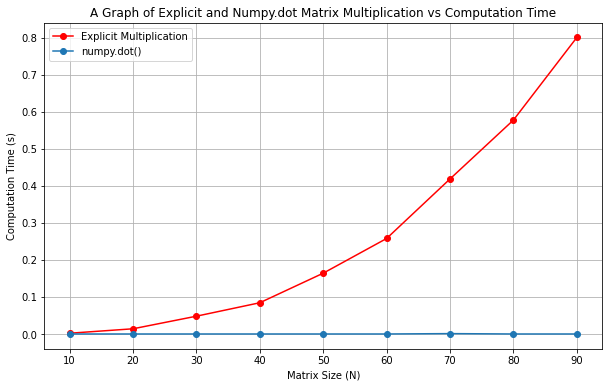
\includegraphics[width=0.7\linewidth]{matrix_multiplication.png}
	\caption{Comparison of Explicit Matrix Multiplication and the Dot Method}
	\label{fig:matrix}
\end{figure}



The results are seen in Figure \ref{fig:matrix}. Indeed, the computational time rises as $N^{3}$ in the for loop method but stays relatively stable at 0 seconds with very little change in the dot method. This shows the difference in computational cost of both methods with the dot method being more computationally efficient.

\section{Question 2}
The isotope $^{213}Bi$ decays to stable $^{209}Bi$ via 2 different routes. \\
\\
\textbf{Route 1:}$^{213}Bi \rightarrow ^{209}Tl \rightarrow ^{209}Pb \rightarrow ^{209}Bi$ \\
\textbf{Route 2:} $^{213}Bi \rightarrow ^{209}Pb \rightarrow ^{209}Bi$ \\
\\
 The half-lives of $^{213}Bi$, $^{209}Tl$ and $^{209}Pb$ are $46 min, 2.2 min$ and $3.3 min$ respectively  and corresponding probabilities of $^{213}Bi$ decaying to $^{209}Tl$ and $^{209}Pb$ being 97.91\%, 2.09\%.
With an initial sample of 10,000 atoms of $^{213}Bi$ , the decay of atoms was simulated by dividing time into slices $\delta t = 1 s$

Each atom of $^{209}Pb$ were randomly decided to decay or not with probability 
\begin{equation}
	p(t) = 1 - 2^{-\frac{t}{\tau}}
	\label{prob}
\end{equation}, where $\tau$ is the half-life of the atom. 

The total number of Lead atoms that decay were counted and subtracted from the number of $^{209}Pb$ initially and added to the number of $^{209}Bi$.

 Likewise, the decaying atoms are counted randomly using the probability obtained from Equation \ref{prob} They are then subtracted from the total number of Thallium atoms and added to the total of $^{209}Pb$. 
 
 For $^{213}Bi$, using the probability of decay from the route it takes randomly, the decayed Bismuth atom number are also counted and are added and subtracted accordingly.

\begin{figure}[!h]
	
		\centering
		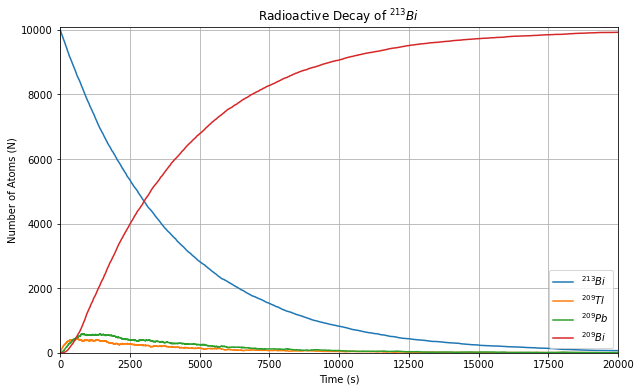
\includegraphics[width=0.7\linewidth]{radio_Bi.png}
		\begin{math}
		\caption{Radioactive Decay Series for $^{213}Bi$}
	\end{math}
			\label{fig:radio_Bi}
	
\end{figure}



These were performed for $t = 20,000 s$ and a graph of Number of atoms against Time was plotted on the same axes as shown in Figure \ref{fig:radio_Bi} It can be seen that the number of $^{213}Bi$ atoms reduce as that of $^{209}Bi$ increase. Also, a few atoms of $^{209}Tl$ and $^{209}Pb$ are created but reduce as time increases as expected due to their lower decay probability values.


\section{Question 3}
The calculation in the decay reaction of the previous question was redone using the transformation method instead.

The probability 
\begin{equation}
	P(t) dt = 2^{-\frac{t}{\tau}} \frac{\ln2}{\tau} dt
	\label{fast_prob}
\end{equation}

N random numbers are generated by drawing from the nonuniform probability distribution in Equation \ref{fast_prob} to represent the time at which each atom decays.
Using the exponential probabilty distribution 
\begin{equation}
	p(x) = \mu \exp(-\mu x)
\end{equation}, with $\mu = \frac{\ln 2}{\tau}$, solving for $x$ gives 
\begin{equation}
	x = -\frac{1}{\mu} \ln(1-z)
	\label{uni_prob}
\end{equation}, where $z$ are uniform random numbers generated in the interval $(0,1)$ 

\begin{figure}[!h]
	
	\centering
	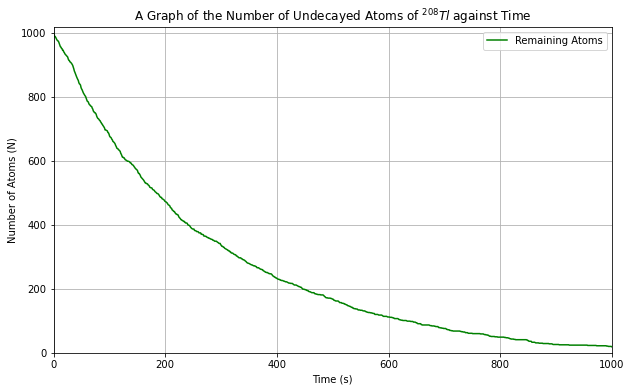
\includegraphics[width=0.7\linewidth]{radio_Tl.png}
	\begin{math}
		\caption{Number of Undecayed atoms of $^{208}Tl$ vs Time}
	\end{math}
	\label{fig:radio_Tl}
	
\end{figure}

1000 random numbers were generated from the nonuniform distribution of Equation \ref{uni_prob} which represents the ties of decay of an equal number of $^{208}Tl$ atoms with a half-life of $3.053 min$. 
A plot of the number of undecayed atoms was plotted as a function of time as seen in Figure \ref{fig:radio_Tl} after being sorted in increasing order.


\section{Question 4}
	The Central Limit Theorem states that the distribution of a normalized version of the sample mean converges to a standard normal distribution. 
	Random variate  
	\begin{equation}
		y = N^{-1} \sum_{i=0}^{N} x_{i}
	\end{equation}, with $x_{i}$ being a random variate distributed as $\exp(-x)$ was generated using the numpy.random package.

\begin{figure}[!h]
	
	\centering
	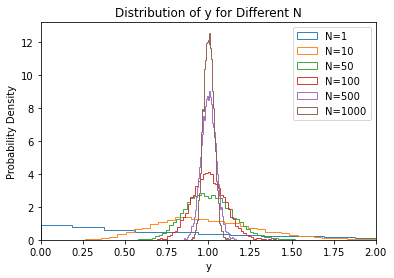
\includegraphics[width=0.73\linewidth]{N_Gaussian.png}
	\caption{Shape of the Distribution as N is increased}
	\label{fig:n_gauss}
	
\end{figure}

As seen in Figure \ref*{fig:n_gauss}, when N is large, the distribution of y tends towards a Gaussian. 

\begin{figure}[!h]
	
	\centering
	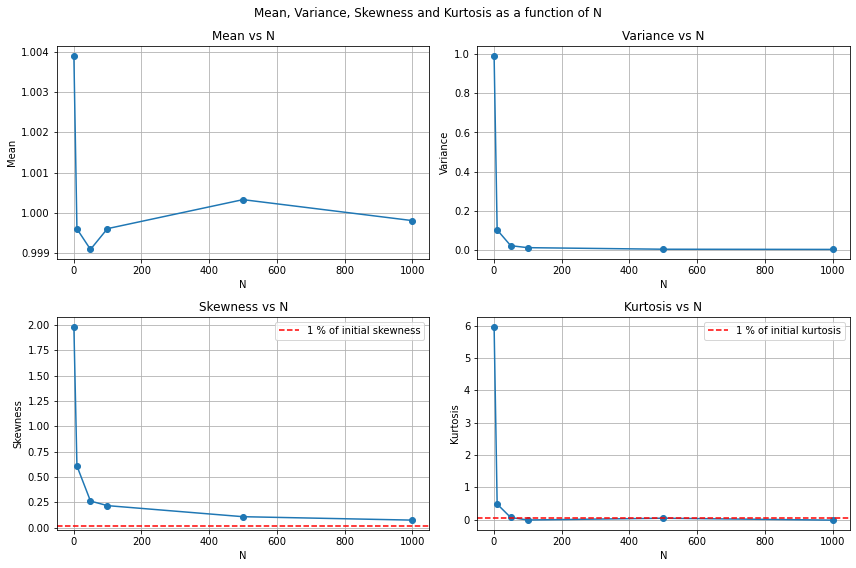
\includegraphics[width=0.98\linewidth]{stats.png}
	\caption{Plots showing the Mean, Vaiance, Skewness and Kurtosis of a Random Distribution}
	\label{fig:stats}
	
\end{figure}


The mean, variance, skewness and kurtosis of the distribution changes as follows from Figure \ref{fig:stats}. The Mean seems to converge at 1, which is the expected value of the mean of an exponential distribution. The variance also converges at 0 which agree with expected analytical results.
	
	It can be estimated from the graph in Figure \ref{fig:stats} that the kurtosis seemed to have reached $1\%$ of its value at about N = 50. The value of the skewness could not be determined form the graph, even when N was increased past 1000.
	
	
\end{document}